\documentclass[tikz,convert={outfile=monoid-in-moncat-associativity.svg}]{standalone}
\begin{document}
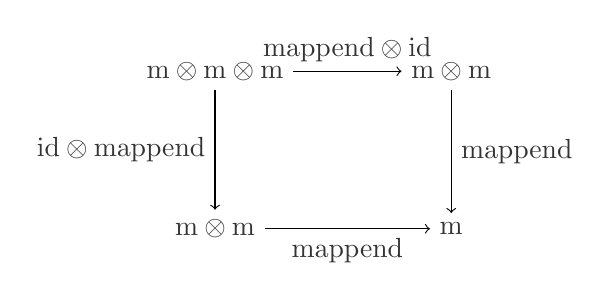
\begin{tikzpicture}
    \node (A) at (0,2) {\textcolor{black!80}{\(\mathrm{m\otimes m\otimes m}\)}};
    \node (B) at (3,2) {\textcolor{black!80}{\(\mathrm{m\otimes m}\)}};
    \node (C) at (0,0) {\textcolor{black!80}{\(\mathrm{m\otimes m}\)}};
    \node (D) at (3,0) {\textcolor{black!80}{\(\mathrm{m}\)}};
    \draw [->] (A) -- node[above] {\textcolor{black!80}{\(\mathrm{mappend\otimes id}\)}} (B); 
    \draw [->] (B) -- node[right] {\textcolor{black!80}{\(\mathrm{mappend}\)}} (D);
    \draw [->] (A) -- node[left] {\textcolor{black!80}{\(\mathrm{id\otimes
    mappend}\)}}  (C);
    \draw [->] (C) -- node[below] {\textcolor{black!80}{\(\mathrm{mappend}\)}} (D);
\end{tikzpicture}
\end{document}
